\section{Ionic Theory and Electrolysis}

\begin{multicols}{2}


%\section*{Ionic Theory} % Moved to Extraction and Properties of Metals, Form III
%
%
%\subsection{Displacement of Copper}
%
%%\begin{center}
%%\includegraphics[width=0.4\textwidth]{./img/.jpg}
%%\end{center}
%
%\begin{description*}
%%\item[Subtopic:]{}
%\item[Materials:]{Steel wool, copper (II) sulphate, water, bottle}
%\item[Setup:]{Prepare a copper (II) sulphate solution by dissolving a spoonful of crystals in about 500 mL of water.}
%\item[Procedure:]{Pour 50 mL of the copper (II) sulphate solution into the container. Dip the steel wool into the solution and observe what happens.}
%%\item[Hazards:]{}
%%\item[Questions:]{}
%\item[Observations:]{A layer of brown copper metal forms on the surface of the steel wool (this is not rust).}
%\item[Theory:]{
%%This is an example of a displacement reaction - metal ions in the solution will reduce and metal solids will oxidize if the proper combination is used. Oxidized compounds lose electrons, while reduced compounds gain electrons. The iron metal oxidizes to form iron (II) ions and the copper (II) ions reduce to form copper metal.
%
%Metals can be arranged according to their reactivity, i.e. how likely they are to form positive ions. A metal higher in the reactivity series will displace a lower metal from a solution. 
%\begin{center}
%K > Na > Ca > Mg > Zn > Fe > Pb > Sn > H > Cu > Ag > Au
%\end{center}
%Iron is higher than copper on the reactivity series, meaning iron ions displace copper ions in solution and the copper ions are deposited as copper metal. $$ \mathrm{CuSO}_{4(aq)} + \mathrm{Fe}_{(s)} \longrightarrow \mathrm{FeSO}_{4(aq)} + \mathrm{Cu(s)} $$}
%%\item[Applications:]{}
%%\item[Notes:]{}
%\end{description*}
%
%%\subsection{Displacement Reaction - Metal Reactivity} % Same as Displacement of Copper
%%
%%%\begin{center}
%%%\includegraphics[width=0.4\textwidth]{./img/.jpg}
%%%\end{center}
%%
%%\begin{description*}
%%%\item[Subtopic:]{}
%%\item[Materials:]{Nail, bottle, copper (II) sulphate}
%%%\item[Setup:]{}
%%\item[Procedure:]{Place the nail at the bottom of a container and cover it with copper (II) sulphate.}
%%%\item[Hazards:]{}
%%%\item[Questions:]{}
%%\item[Observations:]{In 5 minutes a reddish brown precipitate of copper will form.}
%%\item[Theory:]{This is an example of a displacement reaction - metal ions in the solution will reduce and metal solids will oxidize if the proper combination is used. Oxidized compounds lose electrons, while reduced compounds gain electrons. The iron metal oxidizes to form iron (II) ions and the copper (II) ions reduce to form copper metal, precipitating on the nail (this is not rust).}
%%%\item[Applications:]{}
%%\item[Notes:]{Repeat the activity using magnesium sulphate in place copper (II) sulphate. There will be no precipitate this time because the combination of compounds does not yield displacement.}
%%\end{description*}
%
%\subsection{Reactivity Series of Metals}
%
%\begin{center}
%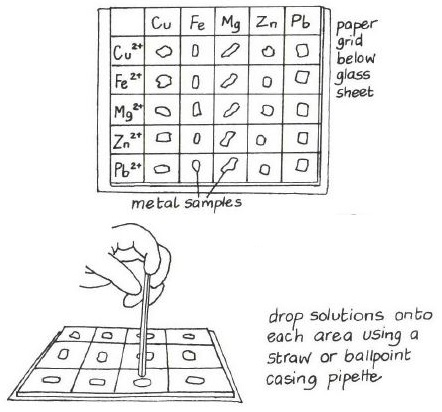
\includegraphics[width=0.4\textwidth]{./img/vso/reactivity-series.jpg}
%\end{center}
%
%\begin{description*}
%%\item[Subtopic:]{}
%\item[Materials:]{Glass sheet, large sheet of paper, metals, solutions of metal ions (see below)}
%\item[Setup:]{Gather and clean small pieces of various metals (e.g.copper wire, iron wool, magnesium ribbon, zinc plate from dry cell, lead shot). Gather some solutions containing metal ions (e.g. copper (II) sulphate, iron (II) sulphate, magnesium sulphate, zinc sulphate, lead nitrate).}
%\item[Procedure:]{Make a grid on the paper as shown. Place the glass sheet over the paper grid. Place the metals on the appropriate squares. Add 2-3 drops of a solution to each metal and observe and change.}
%%\item[Hazards:]{}
%%\item[Questions:]{}
%\item[Observations:]{On some of the squares a black or red (in the
%case of copper displacement) coating is formed
%on the surface of the metal.}
%\item[Theory:]{If a black coating forms on the metal it indicates that the metal ions are being displaced from the solution and deposited onto the metal. This shows that the metal is more reactive than the ion in solution. For example if Fe$^{2+}$ ions in
%solution are dropped onto magnesium, the
%magnesium displaces the Fe$^{2+}$ ions and a black
%coating of iron can be seen on the surface of the
%magnesium.}
%%\item[Applications:]{}
%%\item[Notes:]{}
%\end{description*}
%
%\subsection{Reactivity Rates Analogies}
%
%\begin{center}
%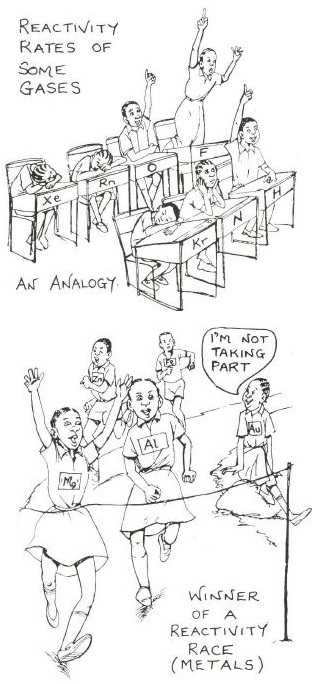
\includegraphics[width=0.4\textwidth]{./img/source/reactivity-rates-cartoons.jpg}
%\end{center}
%
%%\begin{description*}
%%%\item[Subtopic:]{}
%%\item[Materials:]{}
%%\item[Setup:]{}
%%\item[Procedure:]{}
%%\item[Hazards:]{}
%%\item[Questions:]{}
%%\item[Observations:]{}
%%\item[Theory:]{}
%%\item[Applications:]{}
%%\item[Notes:]{}
%%\end{description*}

%==================================================================================================%

\section*{Electrolytes and Non-Electrolytes}


\subsection{Electrolytes}

\begin{center}
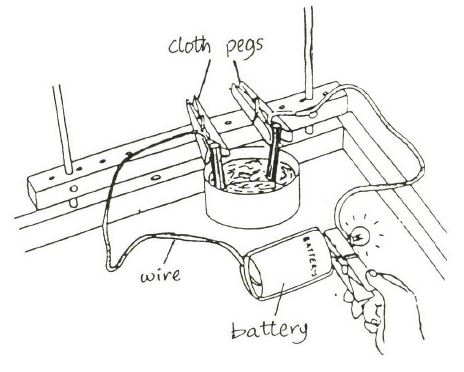
\includegraphics[width=0.45\textwidth]{./img/source/electrolytes.jpg}
\end{center}

\begin{description*}
%\item[Subtopic:]{}
\item[Materials:]{Table salt, distilled water, sugar, vinegar/citric acid, sulphuric acid, bottles, dry cells, clothes pegs, bulb/ammeter, speaker wire, 2 carbon electrodes (from dry cell)}
\item[Setup:]{Connect the circuit in series as shown. Take carbon electrodes from an old dry cell.}
\item[Procedure:]{Place the two carbon electrodes in a container of water. On a piece of paper, pour out some table salt crystals and touch the electrodes to them. Dissolve the salt in the water and again test for conductivity. Repeat with citric acid crystals and solution, then sugar crystals and solution, rinsing the electrodes between tests. Finally test the electrodes in a dilute sulphuric acid solution, rinse, then in vinegar.}
%\item[Hazards:]{}
%\item[Questions:]{}
%\item[Observations:]}
\item[Theory:]{Bubbles of gas at the electrodes indicate the
flow of an electric current. Substances which
conduct electricity in solution are called \emph{electrolytes}. No substance will conduct electricity in the solid state but some of them will
conduct in the dissolved state. Sodium chloride (table salt) is a \emph{strong electrolyte} - the bulb burns brightly. Vinegar and citric acid are \emph{weak electrolyte}s - the bulb burns dimly. Sugar is a \emph{non-electrolyte} - the bulb does not light. The bulb is brighter in sulphuric acid solution than in vinegar even though they are about the same concentration, because the sulphuric acid dissociates completely while citric acid/vinegar only partially dissociate into ions.}
%\item[Applications:]{}
%\item[Notes:]{}
\end{description*}

\subsection{Electrodes}

\begin{center}
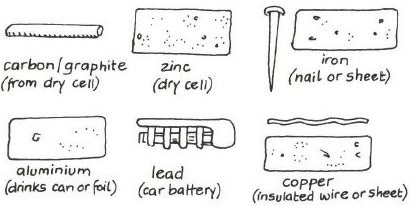
\includegraphics[width=0.45\textwidth]{./img/vso/electrodes.jpg}
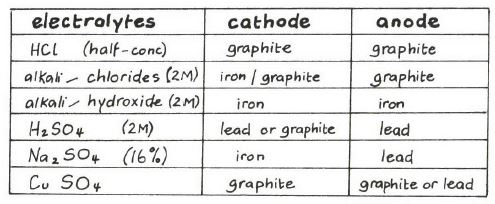
\includegraphics[width=0.45\textwidth]{./img/vso/electrolyte-electrode.jpg}
\end{center}

\begin{description*}
%\item[Subtopic:]{}
%\item[Materials:]{}
%\item[Setup:]{}
%\item[Procedure:]{}
%\item[Hazards:]{}
%\item[Questions:]{}
%\item[Observations:]{}
\item[Theory:]{The materials shown here can be used as electrodes in electrolysis activities. Use the table to find the appropriate matching of electrolyte and electrodes.}
%\item[Applications:]{}
%\item[Notes:]{}
\end{description*}

%\subsection{Electrode Holders} % Put in sources of equip
%
%\begin{center}
%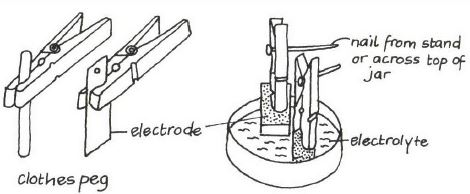
\includegraphics[width=0.4\textwidth]{./img/vso/electrode-holders.jpg}
%\end{center}
%
%\begin{description*}
%%\item[Subtopic:]{}
%\item[Materials:]{}
%\item[Setup:]{}
%\item[Procedure:]{}
%\item[Hazards:]{}
%\item[Questions:]{}
%\item[Observations:]{}
%\item[Theory:]{}
%\item[Applications:]{}
%\item[Notes:]{}
%\end{description*}

\subsection{Electrolysis Setups}

\begin{center}
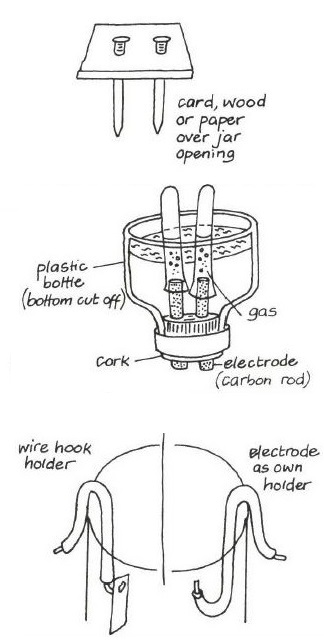
\includegraphics[width=0.49\textwidth]{./img/vso/electrolysis.jpg}
\end{center}

\begin{description*}
%\item[Subtopic:]{}
%\item[Materials:]{}
%\item[Setup:]{}
\item[Procedure:]{Use any of the designs shown for setting up electrolysis experiments.}
%\item[Hazards:]{}
%\item[Questions:]{}
%\item[Observations:]{}
%\item[Theory:]{}
%\item[Applications:]{}
%\item[Notes:]{}
\end{description*}

\subsection{Conservation of Energy} % LASM

\begin{center}
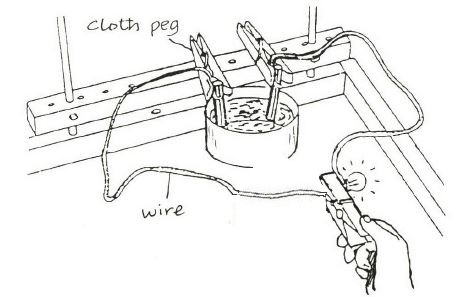
\includegraphics[width=0.45\textwidth]{./img/source/chem-energy.jpg}
\end{center}

\begin{description*}
%\item[Subtopic:]{}
\item[Materials:]{Copper (II) sulphate, zinc metal (from dry cell), copper wire, steel wool, ammeter/bulb}
\item[Setup:]{Prepare a 2 M solution of copper (II) sulphate and clean pieces of copper wire and zinc using steel wool.}
\item[Procedure:]{Connect the zinc anode, ammeter/bulb and copper cathode in series using connecting wires. Dip the zinc and copper electrodes into the copper (II) sulphate solution. Read the current on the ammeter.}
%\item[Hazards:]{}
%\item[Questions:]{}
\item[Observations:]{The ammeter shows a deflection, possibly around 0.05 A.}
\item[Theory:]{The current produced indicates that the chemical energy inherent in the electrodes and the electrolyte solution is converted to electrical energy.}
%\item[Applications:]{}
%\item[Notes:]{}
\end{description*}

%==================================================================================================%

\section*{Mechanism of Electrolysis}


\subsection{Electrolysis of Water} 

\begin{center}
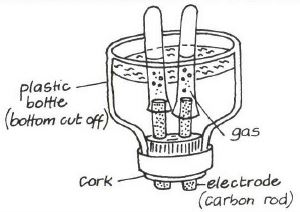
\includegraphics[width=0.4\textwidth]{./img/vso/electrolysis-nacl.jpg}
\end{center}

\begin{description*}
%\item[Subtopic:]{}
\item[Materials:]{Bottle, clothes pegs, dry cells, 2 syringes, speaker wire, bulb, water, table salt}
\item[Setup:]{Remove 2 carbon electrodes from old dry cell batteries. Connect the electrodes and bulb in series with 3-4 dry cells.}
\item[Procedure:]{Fix the electrodes in a cork or bottle top (with super glue to seal). Place an overturned empty syringe tube over each electrode. Fill the container with a dilute sodium chloride solution by dissolving table salt in water. Close the circuit.}
%\item[Hazards:]{}
%\item[Questions:]{}
\item[Observations:]{Bubbles at the electrodes indicate a reaction of electrolysis.}
\item[Theory:]{The cations present are H$^+$ from water and Na$^+$ from the sodium chloride. These migrate to the cathode, where the H$^+$ are discharged because hydrogen is lower than sodium in the reactivity series, and so \emph{hydrogen gas is formed at the cathode}. 

At the anode, OH$^-$ ions from water are discharged in favor of Cl$^-$ ions from salt, and so \emph{oxygen gas is formed at the anode}.

The complete chemical equation for this reaction is:\\
\ce{ 4H+_{(aq)} + 4OH^-_{(aq)} -> 2H2O_{(l)} + O2_{(g)} + 2H2_{(g)} }

The volume of hydrogen gas produced is twice as large as that of oxygen.}
%\item[Applications:]{}
%\item[Notes:]{}
\end{description*}

%==================================================================================================%

%\section*{Laws of Electrolysis} % See LASM

%==================================================================================================%

\section*{Application of Electrolysis}


\subsection{Electroplating}

\begin{center}
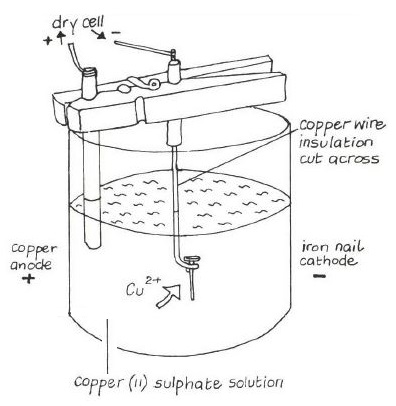
\includegraphics[width=0.45\textwidth]{./img/vso/electroplating.jpg}
\end{center}

\begin{description*}
%\item[Subtopic:]{}
\item[Materials:]{Dry cells, iron nail, copper wire, speaker wire, copper (II) sulphate, water, bottle}
\item[Setup:]{Strip or scrape the insulation from the copper wire as shown and connect to the nail. Connect this end to the \emph{negative} terminal of the dry cell. To the positive terminal connect another stripped piece of copper wire. Place a copper (II) sulphate solution in the container. }
\item[Procedure:]{Submerge the nail and loose copper wire into the solution.}
%\item[Hazards:]{}
%\item[Questions:]{}
\item[Observations:]{In a short time, the nail becomes pinkish as copper deposits on its surface. If left for a long time, the loose copper wire will disappear.}
\item[Theory:]{The copper metal (anode) oxidizes to form Cu$^+$ ions, which migrate towards the cathode (iron nail) where reduction takes place. The copper ions gain electrons to once again form copper metal on the surface of the nail. }
\item[Applications:]{Chrome plating of jewelry, etc. uses this process with chromium in place of copper. Galvanized nails are iron nails with zinc electroplated onto their surface to prevent rusting.}
\item[Notes:]{Use any conducting object in place of the nail, e.g. spoon, graphite electrode, etc.}
\end{description*}


\end{multicols}

\pagebreak